% UCL Thesis LaTeX Template
%  (c) Ian Kirker, 2014
% 
% This is a template/skeleton for PhD/MPhil/MRes theses.
%
% It uses a rather split-up file structure because this tends to
%  work well for large, complex documents.
% We suggest using one file per chapter, but you may wish to use more
%  or fewer separate files than that.
% We've also separated out various bits of configuration into their
%  own files, to keep everything neat.
% Note that the \input command just streams in whatever file you give
%  it, while the \include command adds a page break, and does some
%  extra organisation to make compilation faster. Note that you can't
%  use \include inside an \include-d file.
% We suggest using \input for settings and configuration files that
%  you always want to use, and \include for each section of content.
% If you do that, it also means you can use the \includeonly statement
%  to only compile up the section you're currently interested in.
% You might also want to put figures into their own files to be \input.

% For more information on \input and \include, see:
%  http://tex.stackexchange.com/questions/246/when-should-i-use-input-vs-include


% Formatting rules for theses are here: 
%  http://www.ucl.ac.uk/current-students/research_degrees/thesis_formatting
% Binding and submitting guidelines are here:
%  http://www.ucl.ac.uk/current-students/research_degrees/thesis_binding_submission

% This package goes first and foremost, because it checks all 
%  your syntax for mistakes and some old-fashioned LaTeX commands.
% Note that normally you should load your documentclass before 
%  packages, because some packages change behaviour based on
%  your document settings.
% Also, for those confused by the RequirePackage here vs usepackage
%  elsewhere, usepackage cannot be used before the documentclass
%  command, while RequirePackage can. That's the only functional
%  difference.
\RequirePackage[l2tabu, orthodox]{nag}


% ------ Main document class specification ------
% The draft option here prevents images being inserted,
%  and adds chunky black bars to boxes that are exceeding 
%  the page width (to show that they are).
% The oneside option can optionally be replaced by twoside if
%  you intend to print double-sided. Note that this is
%  *specifically permitted* by the UCL thesis formatting
%  guidelines.
%
% Valid options in terms of type are:
%  phd
%  mres
%  mphil
%\documentclass[12pt,mphil,draft,a4paper,oneside]{ucl_thesis}
\documentclass[12pt,mphil,a4paper,oneside]{ucl_thesis}


% Package configuration:
%  LaTeX uses "packages" to add extra commands and features.
%  There are quite a few useful ones, so we've put them in a 
%   separate file.
% -------- Packages --------

% This package just gives you a quick way to dump in some sample text.
% You can remove it -- it's just here for the examples.
\usepackage{blindtext}

% This package means empty pages (pages with no text) won't get stuff
%  like chapter names at the top of the page. It's mostly cosmetic.
\usepackage{emptypage}

% The graphicx package adds the \includegraphics command,
%  which is your basic command for adding a picture.
\usepackage{graphicx}

% This command is provided by the graphicx package, and 
%  controls the default dpi resolution of images you use.
%  72 is the default, but 300 is more normal, and 600 is
%  as good as you can expect to be able to get on normal paper.
\pdfimageresolution=300


% The float package improves LaTeX's handling of floats,
%  and also adds the option to *force* LaTeX to put the float
%  HERE, with the [H] option to the float environment.
\usepackage{float}

% The amsmath package enhances the various ways of including
%  maths, including adding the align environment for aligned
%  equations.
\usepackage{amsmath}

% Use these two packages together -- they define symbols
%  for e.g. units that you can use in both text and math mode.
\usepackage{gensymb}
\usepackage{textcomp}
% You may also want the units package for making little
%  fractions for unit specifications.
%\usepackage{units}


% The setspace package lets you use 1.5-sized or double line spacing.
\usepackage{setspace}
\setstretch{1.5}

% That just does body text -- if you want to expand *everything*,
%  including footnotes and tables, use this instead:
%\renewcommand{\baselinestretch}{1.5}


% PGFPlots is either a really clunky or really good way to add graphs
%  into your document, depending on your point of view.
% There's waaaaay too much information on using this to cover here,
%  so, you might want to start here:
%   http://pgfplots.sourceforge.net/
%  or here:
%   http://pgfplots.sourceforge.net/pgfplots.pdf
%\usepackage{pgfplots}
%\pgfplotsset{compat=1.3} % <- this fixed axis labels in the version I was using

% PGFPlotsTable can help you make tables a little more easily than
%  usual in LaTeX.
% If you're going to have to paste data in a lot, I'd suggest using it.
%  You might want to start with the manual, here:
%  http://pgfplots.sourceforge.net/pgfplotstable.pdf
%\usepackage{pgfplotstable}

% These settings are also recommended for using with pgfplotstable.
%\pgfplotstableset{
%	% these columns/<colname>/.style={<options>} things define a style
%	% which applies to <colname> only.
%	empty cells with={--}, % replace empty cells with '--'
%	every head row/.style={before row=\toprule,after row=\midrule},
%	every last row/.style={after row=\bottomrule}
%}


% The mhchem package provides chemistry formula typesetting commands
%  e.g. \ce{H2O}
%\usepackage[version=3]{mhchem}

% And the chemfig package gives a weird command for adding Lewis 
%  diagrams, for e.g. organic molecules
%\usepackage{chemfig}

% The linenumbers command from the lineno package adds line numbers
%  alongside your text that can be useful for discussing edits 
%  in drafts.
% Remove or comment out the command for proper versions.
%\usepackage[modulo]{lineno}
% \linenumbers 


% Alternatively, you can use the ifdraft package to let you add
%  commands that will only be used in draft versions
%\usepackage{ifdraft}

% For example, the following adds a watermark if the draft mode is on.
%\ifdraft{
%  \usepackage{draftwatermark}
%  \SetWatermarkText{\shortstack{\textsc{Draft Mode}\\ \strut \\ \strut \\ \strut}}
%  \SetWatermarkScale{0.5}
%  \SetWatermarkAngle{90}
%}


% The multirow package adds the option to make cells span 
%  rows in tables.
\usepackage{multirow}


% Subfig allows you to create figures within figures, to, for example,
%  make a single figure with 4 individually labeled and referenceable
%  sub-figures.
% It's quite fiddly to use, so check the documentation.
%\usepackage{subfig}

% The natbib package allows book-type citations commonly used in
%  longer works, and less commonly in science articles (IME).
% e.g. (Saucer et al., 1993) rather than [1]
% More details are here: http://merkel.zoneo.net/Latex/natbib.php
%\usepackage{natbib}

% The bibentry package (along with the \nobibliography* command)
%  allows putting full reference lines inline.
%  See: 
%   http://tex.stackexchange.com/questions/2905/how-can-i-list-references-from-bibtex-file-in-line-with-commentary
\usepackage{bibentry} 

% The isorot package allows you to put things sideways 
%  (or indeed, at any angle) on a page.
% This can be useful for wide graphs or other figures.
%\usepackage{isorot}

% The caption package adds more options for caption formatting.
% This set-up makes hanging labels, makes the caption text smaller
%  than the body text, and makes the label bold.
% Highly recommended.
\usepackage[format=hang,font=small,labelfont=bf]{caption}

% If you're getting into defining your own commands, you might want
%  to check out the etoolbox package -- it defines a few commands
%  that can make it easier to make commands robust.
\usepackage{etoolbox}

\usepackage{amsmath}
\usepackage{bm}
\usepackage{xcolor, colortbl}
\usepackage{amsmath,amscd,amsbsy,amssymb,latexsym,url,bm}
\usepackage{amssymb}
\usepackage{longtable}
\usepackage{multirow}
\usepackage{subcaption}
\usepackage{algorithm} 
\usepackage{algpseudocode}



% Sets up links within your document, for e.g. contents page entries
%  and references, and also PDF metadata.
% You should edit this!
%%
%% This file uses the hyperref package to make your thesis have metadata embedded in the PDF, 
%%  and also adds links to be able to click on references and contents page entries to go to 
%%  the pages.
%%

% Some hacks are necessary to make bibentry and hyperref play nicely.
% See: http://tex.stackexchange.com/questions/65348/clash-between-bibentry-and-hyperref-with-bibstyle-elsart-harv
\usepackage{bibentry}
\makeatletter\let\saved@bibitem\@bibitem\makeatother
\usepackage[pdftex,hidelinks]{hyperref}
\makeatletter\let\@bibitem\saved@bibitem\makeatother
\makeatletter
\AtBeginDocument{
    \hypersetup{
        pdfsubject={Thesis Subject},
        pdfkeywords={Thesis Keywords},
        pdfauthor={Author},
        pdftitle={Title},
    }
}
\makeatother
    


% And then some settings in separate files.
% These settings are from:
%  http://mintaka.sdsu.edu/GF/bibliog/latex/floats.html

% They give LaTeX more options on where to put your figures, and may
%  mean that fewer of your figures end up at the tops of pages far
%  away from the thing they're related to.

% Alters some LaTeX defaults for better treatment of figures:
% See p.105 of "TeX Unbound" for suggested values.
% See pp. 199-200 of Lamport's "LaTeX" book for details.

%   General parameters, for ALL pages:
\renewcommand{\topfraction}{0.9}	% max fraction of floats at top
\renewcommand{\bottomfraction}{0.8}	% max fraction of floats at bottom

%   Parameters for TEXT pages (not float pages):
\setcounter{topnumber}{2}
\setcounter{bottomnumber}{2}
\setcounter{totalnumber}{4}     % 2 may work better
\setcounter{dbltopnumber}{2}    % for 2-column pages
\renewcommand{\dbltopfraction}{0.9}	% fit big float above 2-col. text
\renewcommand{\textfraction}{0.07}	% allow minimal text w. figs

%   Parameters for FLOAT pages (not text pages):
\renewcommand{\floatpagefraction}{0.7}	% require fuller float pages
% N.B.: floatpagefraction MUST be less than topfraction !!
\renewcommand{\dblfloatpagefraction}{0.7}	% require fuller float pages

% remember to use [htp] or [htpb] for placement,
% e.g. 
%  \begin{figure}[htp]
%   ...
%  \end{figure} % For things like figures and tables
\bibliographystyle{unsrt}   % For bibliographies

% Title Settings
\setcounter{secnumdepth}{3}
\setcounter{tocdepth}{3}
\title{A Thesis Title}
\author{Author Name}
\department{Department of Something}


\begin{document}



\nobibliography*
% This is a dumb trick that works with the bibentry package to let
%  you put bibliography entries whereever you like.
% I used this to put references to papers a chapter's work was 
%  published in at the end of that chapter.
% For more information, see: http://stefaanlippens.net/bibentry

% If you haven't finished making your full BibTex file yet, you
%  might find this useful -- it'll just replace all your
%  citations with little superscript notes.
% Uncomment to use.
%\renewcommand{\cite}[1]{\emph{\textsuperscript{[#1]}}}

% At last, content! Remember filenames are case-sensitive and 
%  *must not* include spaces.
\maketitle
\makedeclaration

\begin{abstract} % 300 word limit
We consider in RTB display advertising how advertisers actively bid an impression considering a long-term objective. It is a combination of CTR estimation and repeated auctions. First, we use the CTR prediction models to find the distribution of market price estimator and then we deal with a reinforcement learning problem to maximise the total utility during the finite sequential auctions. Three CTR prediction models are applied here to obtain the estimator. FFM usually has the better performance than BOPR and FTRL. The ensemble of these three predictors can lead to more effective performance. Our analysis shows that in the second price auction with a logistic click-through model, the optimal bid strategy is not to bid the true value but bid a higher price than it in a finite sequential process. In the end, after advertisers obtain enough information and feedbacks from the market, the bidding price will converge to their true value and it becomes a one-shot auction with side information.
\end{abstract}

\begin{acknowledgements}
First and foremost I would like to sincerely thank my project supervisor Dr. Jun Wang who always had time for me. Without his invaluable advice, guidance and supervision, the quality of this thesis cannot reach such high satisfaction. I appreciate the wisdom of his way in both technical and theoretical perspectives that motivated me to think forward and concentrate on my project deeply. His academic rigor, enthusiasm and strong sense of responsibility are the most valuable characters I learnt during the period. Besides, I really want to thank PhD student and also my good friend Weinan Zhang who gave me many useful suggestions for the project. His patience and professional skills left me an unforgettable impression. I would also like to thank my personal tutor Dr. Massimiliano Pontil for his tutorials throughout my entire MSc course. Most of all, heartfelt thanks must go to my parents and my family. They have offered me unconditional support and encouragement since I went to master study at UCL. Thank for their company through both the highs and lows of my experience. They are the most important and wonderful treasure in my life forever.
\end{acknowledgements}

\setcounter{tocdepth}{2} 
% Setting this higher means you get contents entries for
%  more minor section headers.

\tableofcontents
\listoffigures
\listoftables


\include{Introduction}
\chapter{Click-through Rate (CTR) Prediction}
\label{chapterlabel2}

In this chapter, we describe the dataset that we use for CTR prediction and then introduce some preprocessing and feature engineering techniques. Three advanced and practical models are included. They are Bayesian Online Probit Regression (BOPR), Follow the Regularized Leader (FTRL) and Field-aware Factorization Machine (FFM) respectively. The following Figure~\ref{fig:flowchart} is the workflow of the CTR estimation.

\begin{figure}[h]
\centering
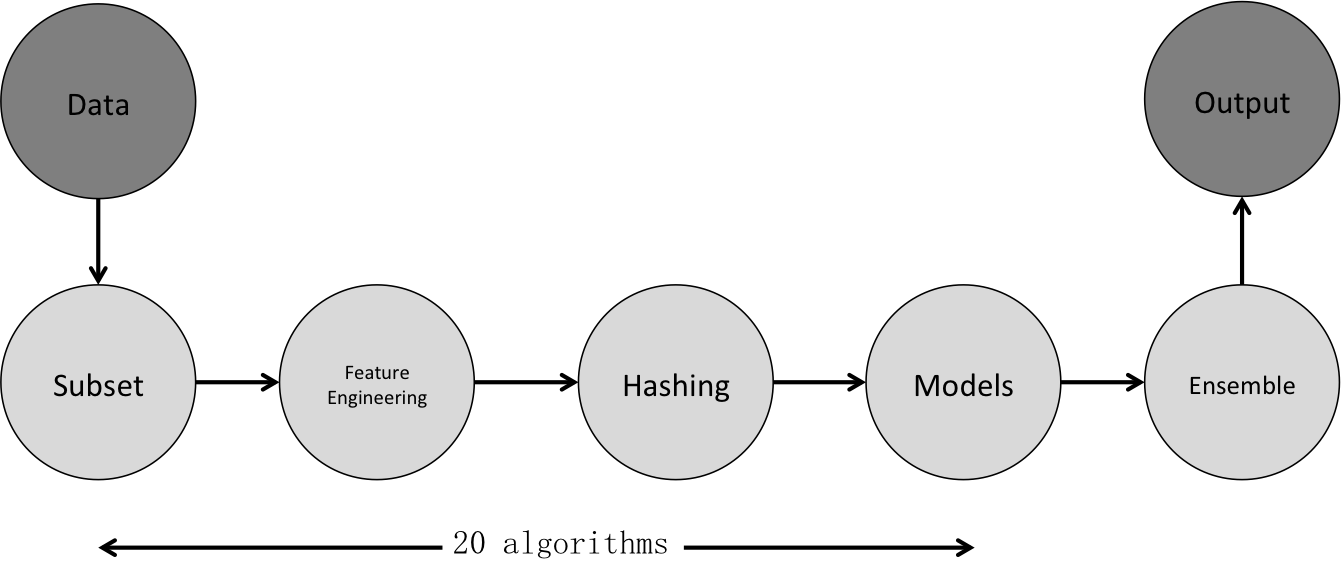
\includegraphics[width=0.9\textwidth]{flowchart.png}
\caption{The work flow chart of CTR estimation procedure}
\label{fig:flowchart}
\end{figure}

\section{Origins of Data Features}
RTB is a well-studied problem in online advertising as most of researches only limit to keyword auction in the context of sponsored search. It is fundamentally different and based on a second price auction \cite{williamvickrey1961}, which has recently emerged as a new display advertising paradigm \cite{zhang2015statistical, zhang2014real, Zhang:2014:ORB:2623330.2623633}. Unlike traditional sponsored search or contextual advertising, where an advertiser presets a bid price for each keyword chosen for their campaigns, advertisers bid for each given impression in RTB. The process takes less than 100ms time frame. Besides, RTB is a type of programmatic buying, which means automated the buying, placement and optimization of ad inventory. Comparing to RTB, some publishers sell their inventory in advance with a fixed price. The bidding price is based on Key Performance Indicator (KPI) like CTR. The whole process is an auction game \cite{zhang2014real}.

The payment and revenue formally consists of three elements: Page View (PV), Click-through Rate (CTR) and Cost per Click (CPC). CTR will be used for the valuation of ads for advertisers and revenue model of ads for publishers. As a consequence, the management of CTR is absolutely crucial to advertising and its corresponding business value.

In this project, we use the RTB data from iPinYou as our training and test dataset. The dataset includes 26 features shown in Table~\ref{tab:features}.

\begin{table}[h]
\caption{The log data format of iPinYou dataset.}
\label{tab:features}
\begin{center}
\begin{tabular}{ l l l } 
\hline
Col & Description & Example \\
\hline
1 & Bid ID & 0150008...3g4fa5621 \\ 
2 & Timestamp & 20129220001004721 \\ 
3 & Log type & 1 \\ 
4 & iPinYou ID & 48598757396839735 \\
5 & User-Agent & windows-chrome \\
6 & IP & 117.86.123.* \\
7 & Region & 16 \\
8 & City & 11 \\
9 & Ad exchange & 1 \\
10 & Domain & trqRTvNNQIj7gspy \\
11 & URL & bebefa5efe83...45e7c50b \\
12 & Anonymous URL ID & null \\
13 & Ad slot ID & 3582857028 \\
14 & Ad slot width & 336 \\
15 & Ad slot height & 280 \\
16 & Ad slot visibility & 2 \\
17 & Ad slot format & 0 \\
18 & Ad slot floor price & 5 \\
19 & Creative ID & 778d3...16d68ad923a1 \\
20 & Bidding price & 300 \\
21 & Paying price & 118 \\
22 & Key page URL & bebefa5ef...45e7c5085b \\
23 & Advertiser ID & 1458 \\
24 & User Tags & 13042,10057,10006 \\
25 & Weekday & 6 \\
26 & Hour & 0 \\
\hline
\end{tabular}
\end{center}
\end {table}

In general,  the auction and ad features (all columns except 3, 20 and 21) are categorical data that are sent to bidding engine to make a bid response. The auction winning price (column 21) is a numerical integer. If the highest price is larger this, the Demand side platform (DSP) will win this impression. The user feedback (click and conversion) on this ad impression (column 3) is the target of the dataset. As we mainly focus on the prediction of CTR, the label is a binary number. The clickability of the ad depends on the type of ad and user. It is not relevant to the bidding aspect. Thus, the data we use to estimate CTR model is a categorical input. Table~\ref{tab:Advertiser} shows the summary of advertiser diversity. The advertiser from different field has various bidding behavior.

\begin{table}[H]
\caption{Advertiser fields and statistics}
\label{tab:Advertiser}
\begin{center}
\begin{tabular}{ l l l l l l l l l } 
\hline
Advertiser ID & Season & Period & Bids & Impressions & Clicks & CTR \\
\hline
1458 & 2 & 6-12 Jun & 14,701,496 & 3,083,056 & 2,454 & 0.080\% \\
2259 & 3 & 19-22 Oct & 2,987,731 & 835,556 & 280 & 0.034\% \\
2261 & 3 & 24-27 Oct & 2,159,708 & 687,617 & 207 & 0.030\% \\
2821 & 3 & 21-23 Oct & 5,292,053 & 1,322,561 & 843 & 0.064\% \\
2997 & 3 & 23-26 Oct & 1,017,927 & 312,437 & 1,386 & 0.444\% \\
3358 & 2 & 6-12 Jun & 3,751,016 & 1,742,104 & 1,358 & 0.078\% \\
3386 & 2 & 6-12 Jun & 14,091,931 & 2,847,802 & 2,076 & 0.073\% \\
3427 & 2 & 6-12 Jun & 14,032,619 & 2,593,765 & 1,926 & 0.074\% \\
3476 & 2 & 6-12 Jun & 6,712,268 & 1,970,360 & 1,027 & 0.052\% \\
Total & 2,3 & - & 64,746,749 & 15,395,258 & 11,557 & 0.075\% \\
\hline
\end{tabular}
\end{center}
\end {table}

We display basic statistics based on user feedback on advertisers of training dataset. Specifically, they are the mean value with the standard error of CTR against some features, such as weekday, hour, user agent, region, city, slot size and ad exchange, etc. From Figure~\ref{fig:advertiserstatistics}, we can see that different advertisers have various users' preference, which results in different impact on CTR.

\begin{figure}[htbp]

\begin{subfigure}{0.5\textwidth}
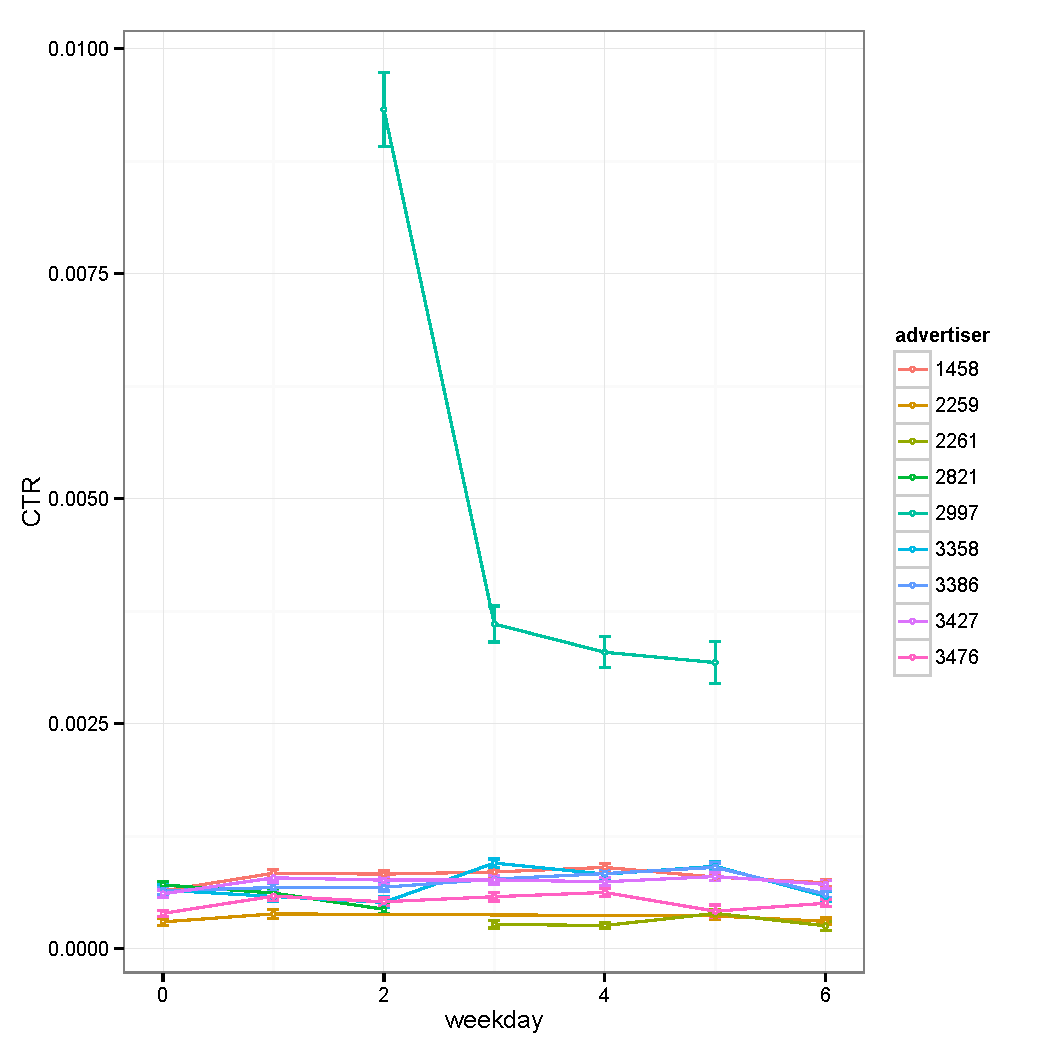
\includegraphics[width=0.9\linewidth, height=5cm]{weekday.pdf}
\caption{Weekday}
\label{fig:weekday}
\end{subfigure}
\begin{subfigure}{0.5\textwidth}
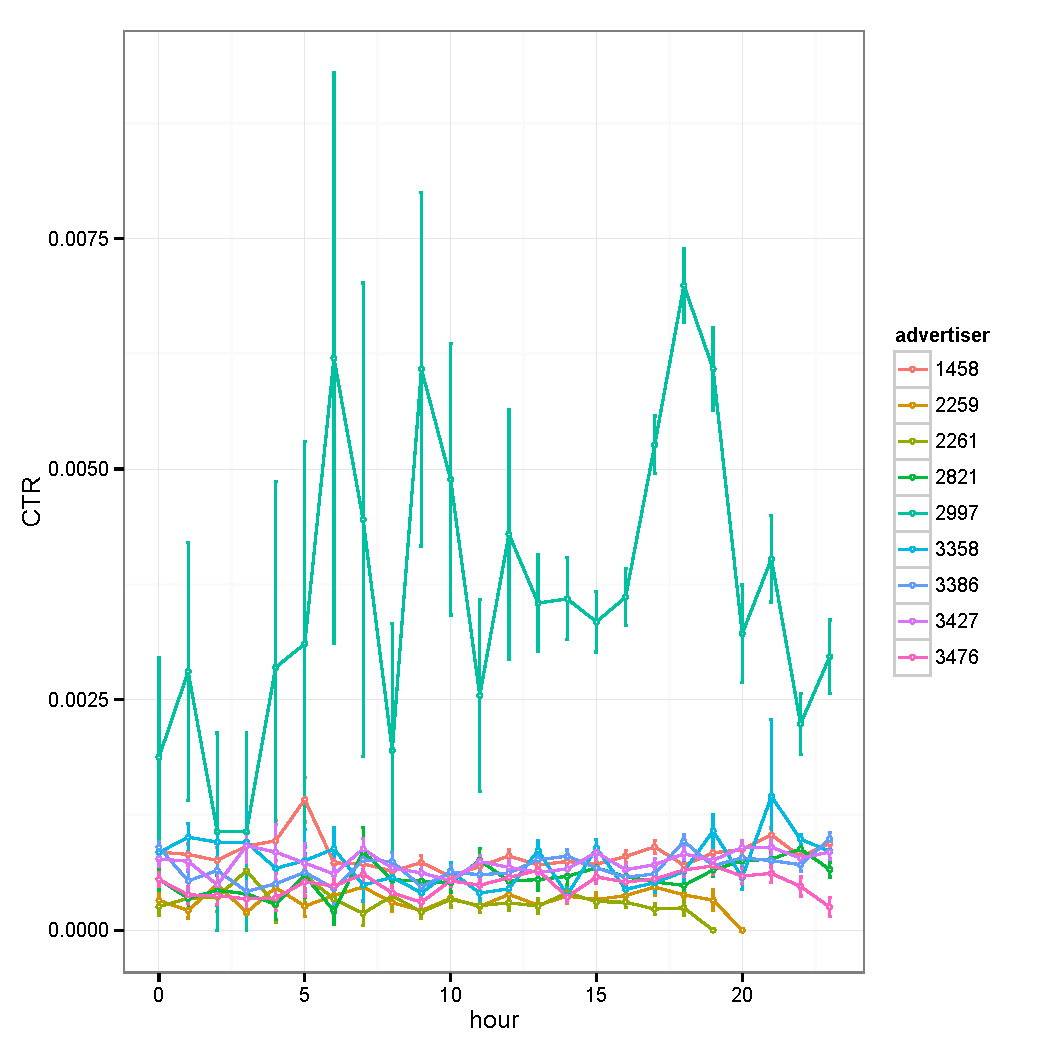
\includegraphics[width=0.9\linewidth, height=5cm]{hour.pdf}
\caption{Hour}
\label{fig:hour}
\end{subfigure}
\begin{subfigure}{0.5\textwidth}
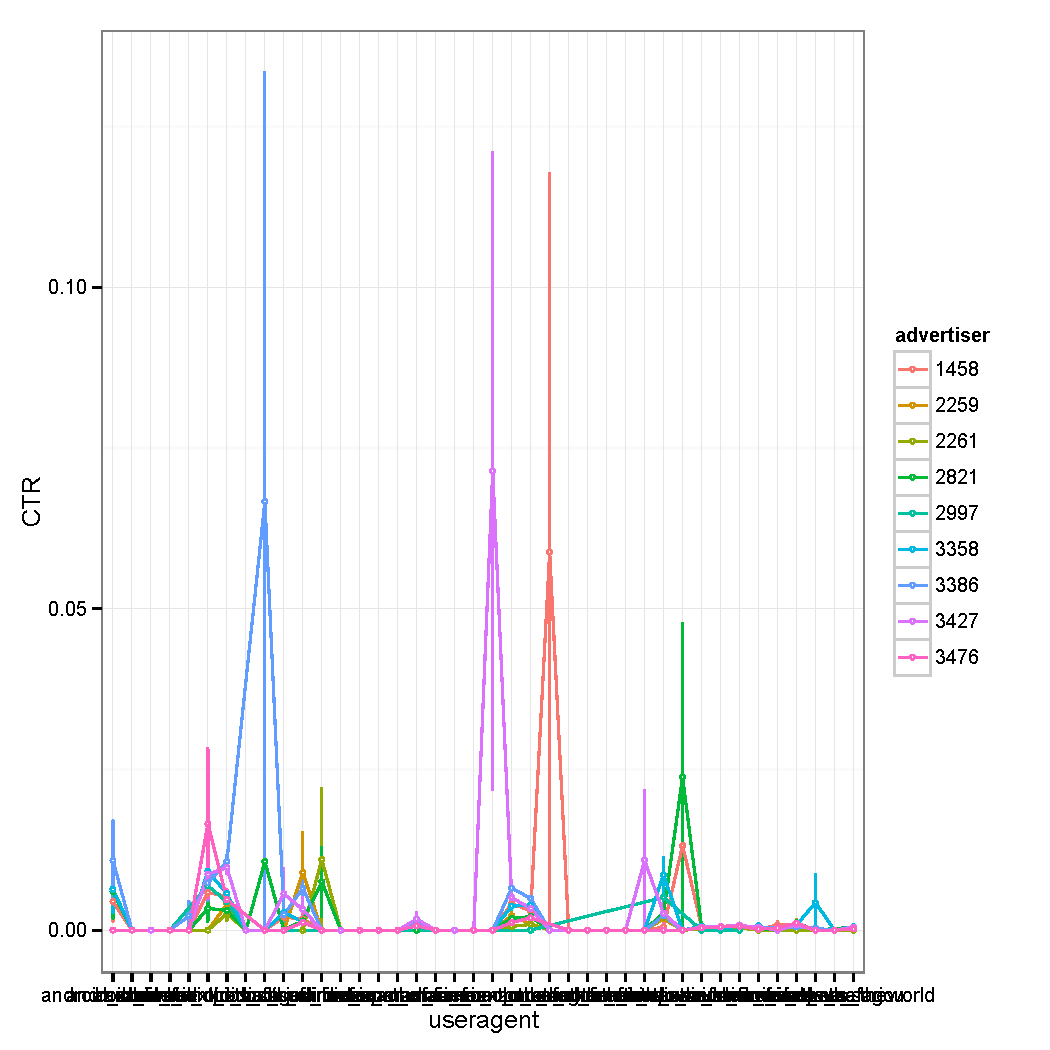
\includegraphics[width=0.9\linewidth, height=5cm]{useragent.pdf}
\caption{Useragent}
\label{fig:useragent}
\end{subfigure}
\begin{subfigure}{0.5\textwidth}
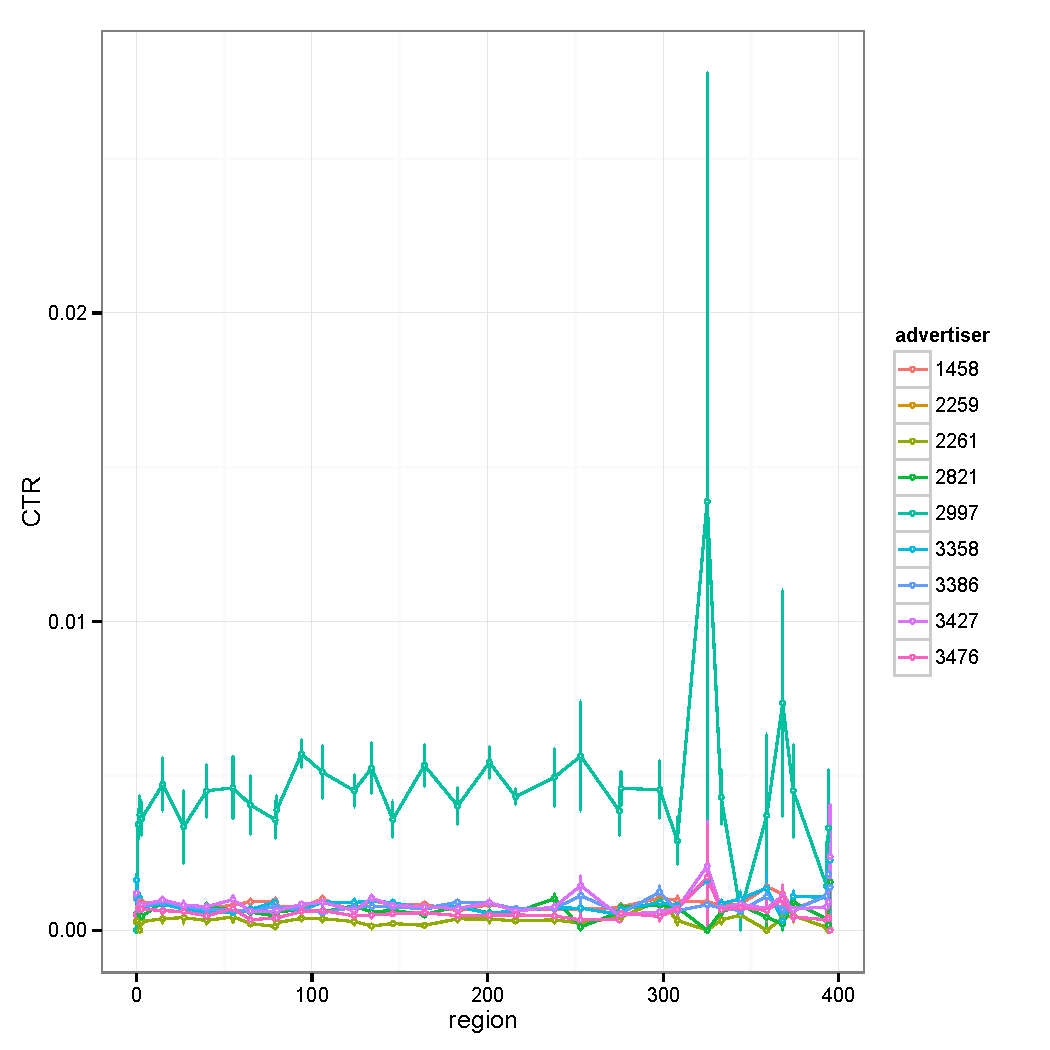
\includegraphics[width=0.9\linewidth, height=5cm]{region.pdf}
\caption{Region}
\label{fig:region}
\end{subfigure}
\begin{subfigure}{0.5\textwidth}
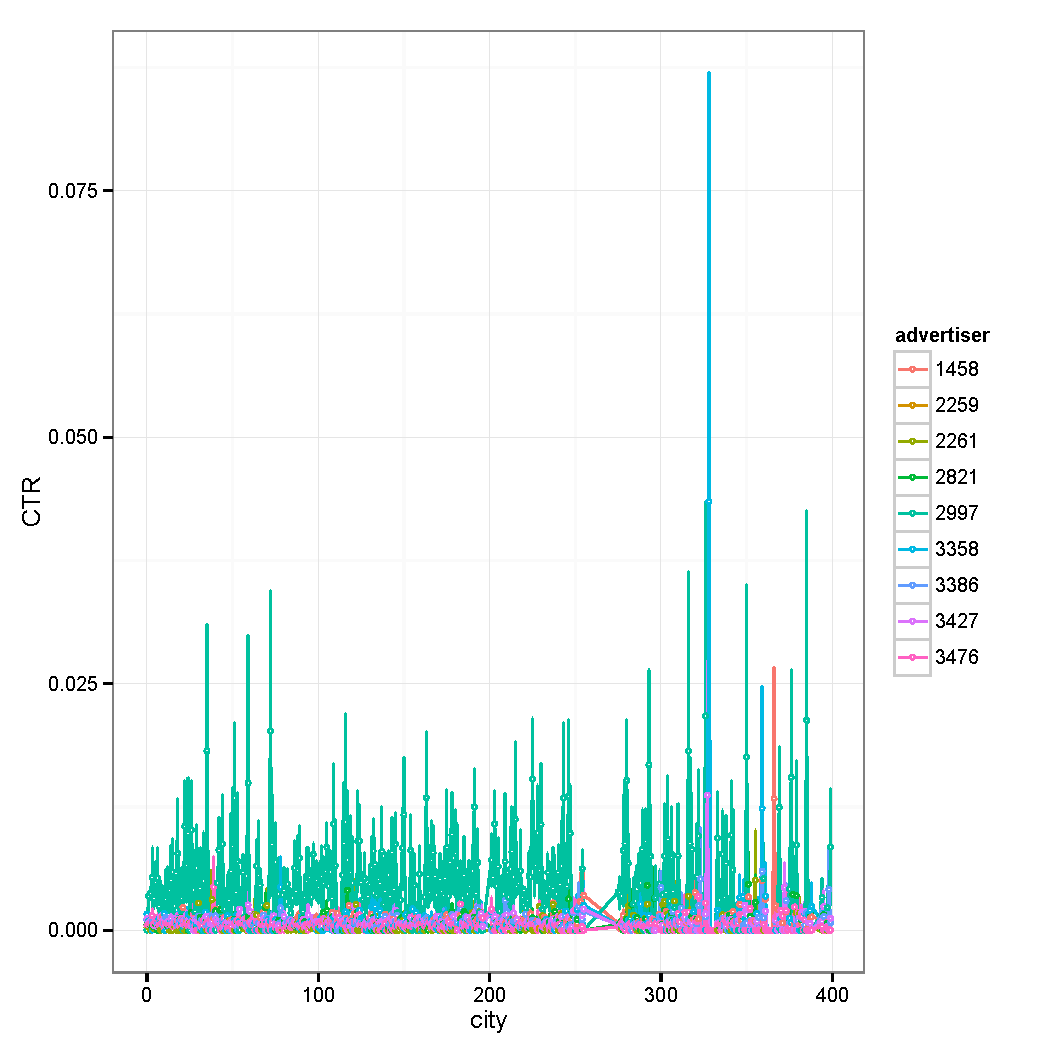
\includegraphics[width=0.9\linewidth, height=5cm]{city.pdf}
\caption{City}
\label{fig:city}
\end{subfigure}
\begin{subfigure}{0.5\textwidth}
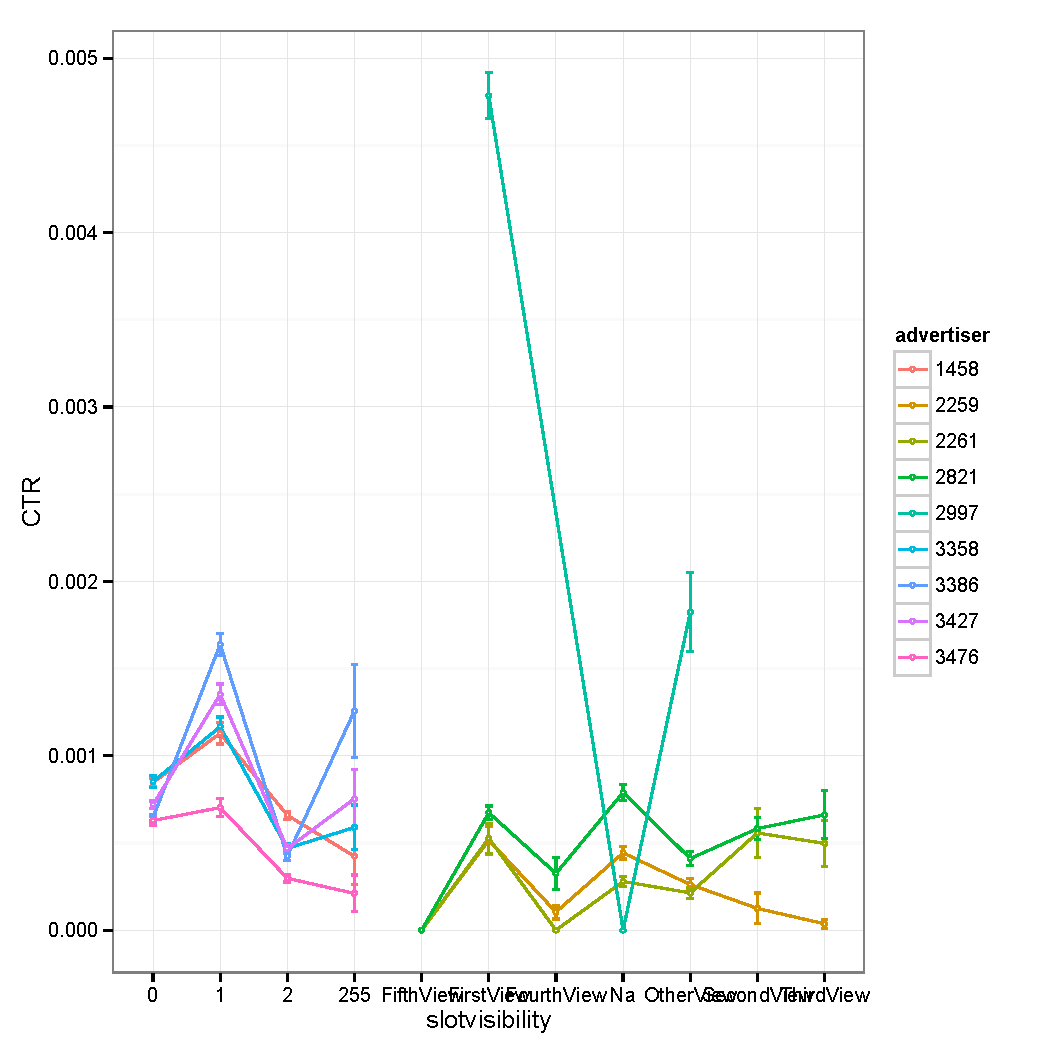
\includegraphics[width=0.9\linewidth, height=5cm]{visibility.pdf}
\caption{Visibility}
\label{fig:visibility}
\end{subfigure}
\begin{subfigure}{0.5\textwidth}
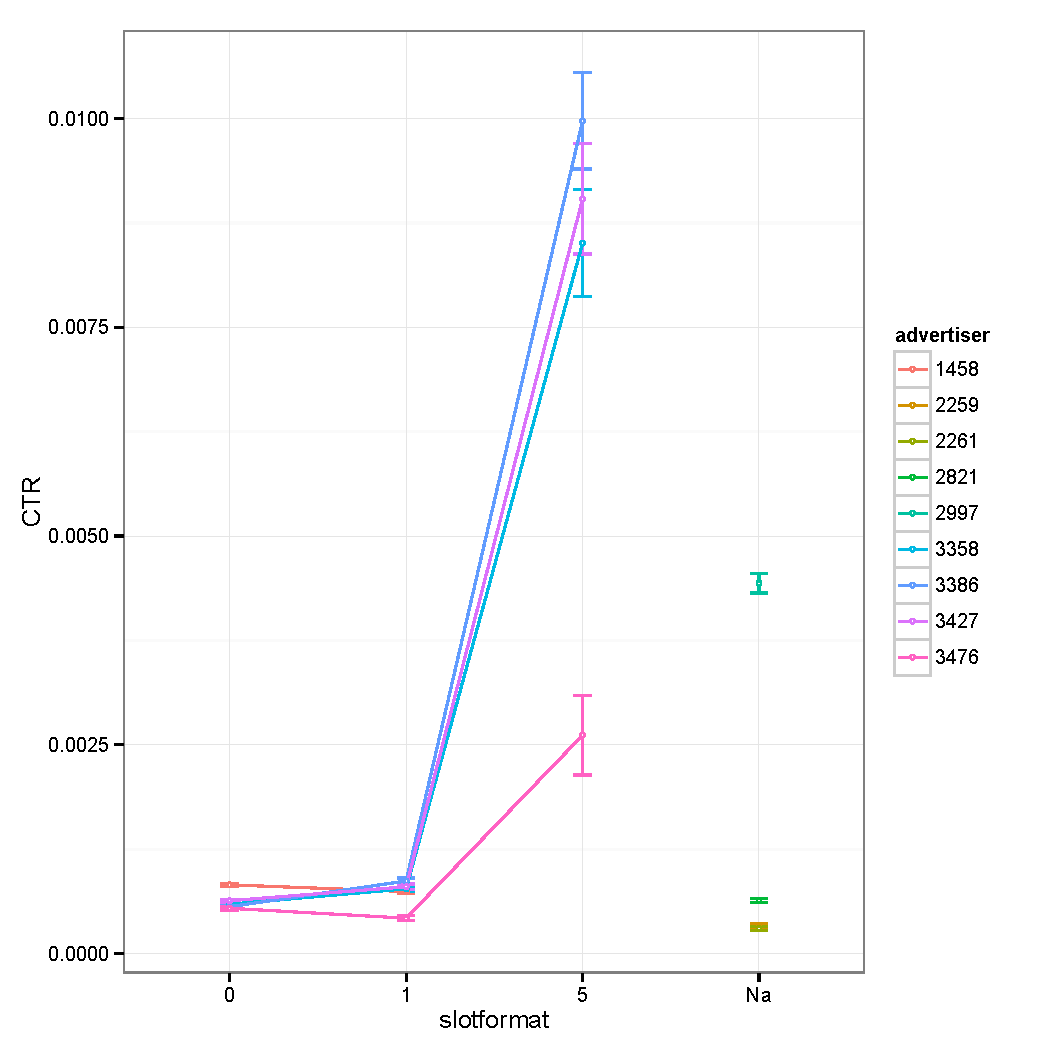
\includegraphics[width=0.9\linewidth, height=5cm]{format.pdf}
\caption{Format}
\label{fig:format}
\end{subfigure}
 \begin{subfigure}{0.5\textwidth}
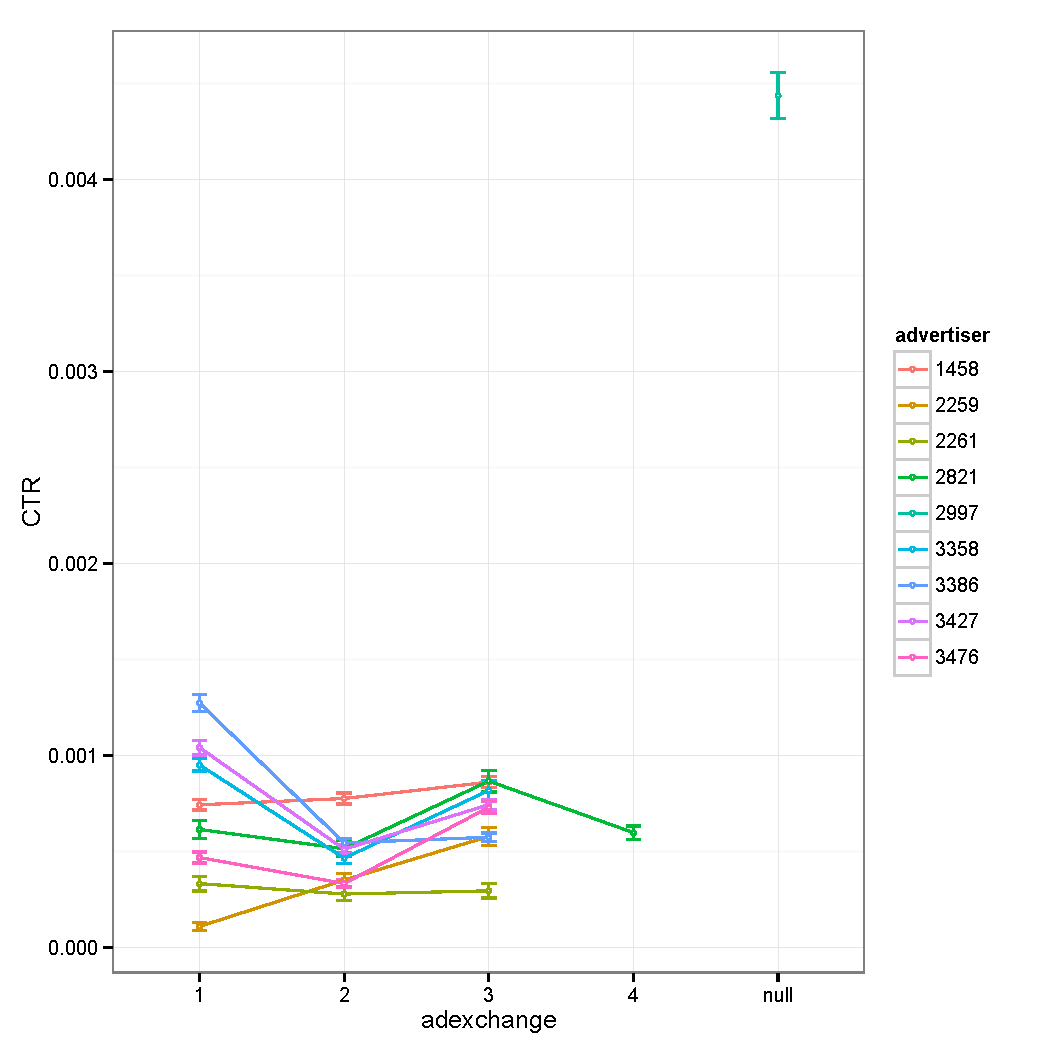
\includegraphics[width=0.9\linewidth, height=5cm]{exchange.pdf}
\caption{Exchange}
\label{fig:exchange}
\end{subfigure}

\caption{CTR distribution against different features of all advertisers}
\label{fig:advertiserstatistics}
\end{figure}

\section{Preprocessing and Feature Engineering}

Except the original categorical features, we can use tree model like \emph{Random Forest} (RF) and \emph{Gradient Boosting Descent Tree} (GBDT) to generate new features. Adding high order combination features is a variant and trick to better predicting performance. This approach is proposed by Facebook \cite{xinranhejunfengpanetc2014}. The details of RF and GBDT can refer to \cite{jeromeh.friedman1999}. A concrete example of implementation is shown in Figure~\ref{fig:GBDT}. Assume that we have already trained GBDT with 3 trees with depth 2. We feed an impression $\mathbf{x}$ into these trees. The first tree thinks $\mathbf{x}$ belong to node 4, the second node 7, and the third node 6. Then we generate a new feature 1:4 2:7 3:6 for this impression.

\begin{figure}[htbp]
\centering
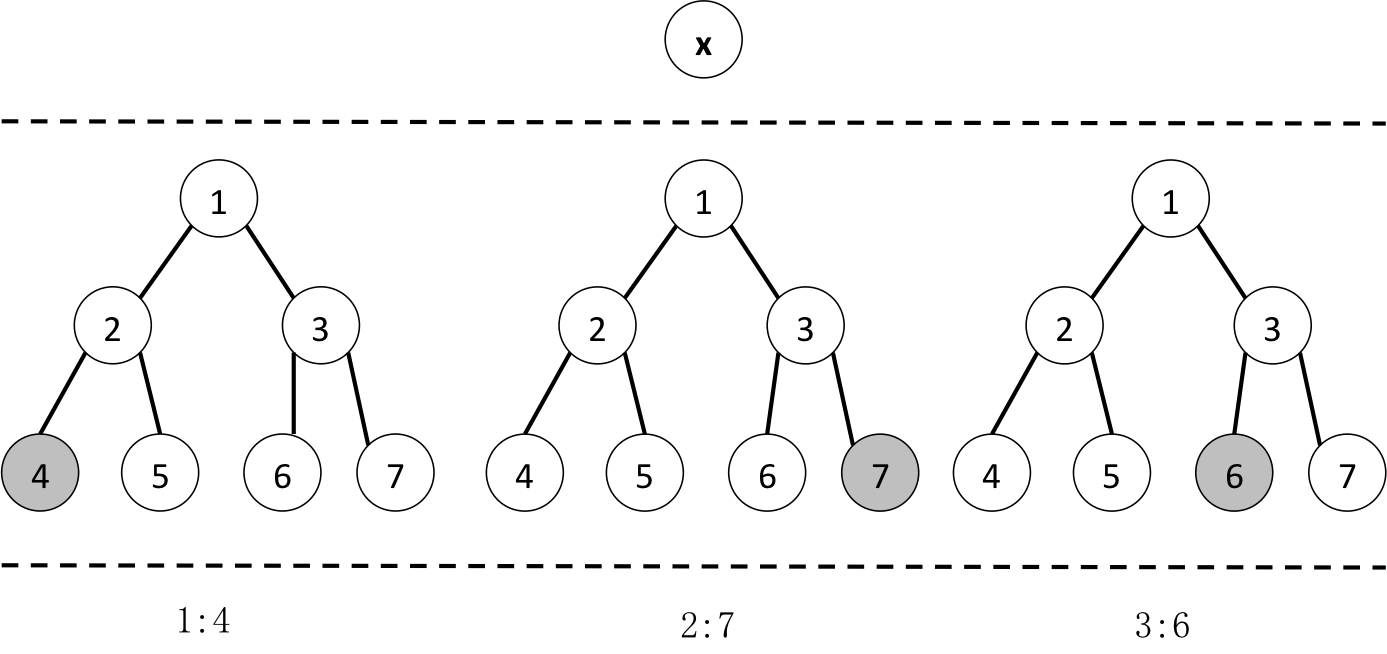
\includegraphics[width=0.8\textwidth]{GBDT.png}
\caption{The GBDT can be used to generate new features}
\label{fig:GBDT}
\end{figure}

The representational power of deep interaction-product network is usually applied to deep learning in speech recognition and computer vision. The dimension of feature is extremely high in computational advertisement if considering all feature interaction. Suppose we have $N$ single features, the candidate of combination of features will be $2^{N}$. The sparse learning algorithm cannot learn parameters properly. 

\begin{figure}[htbp]
\centering
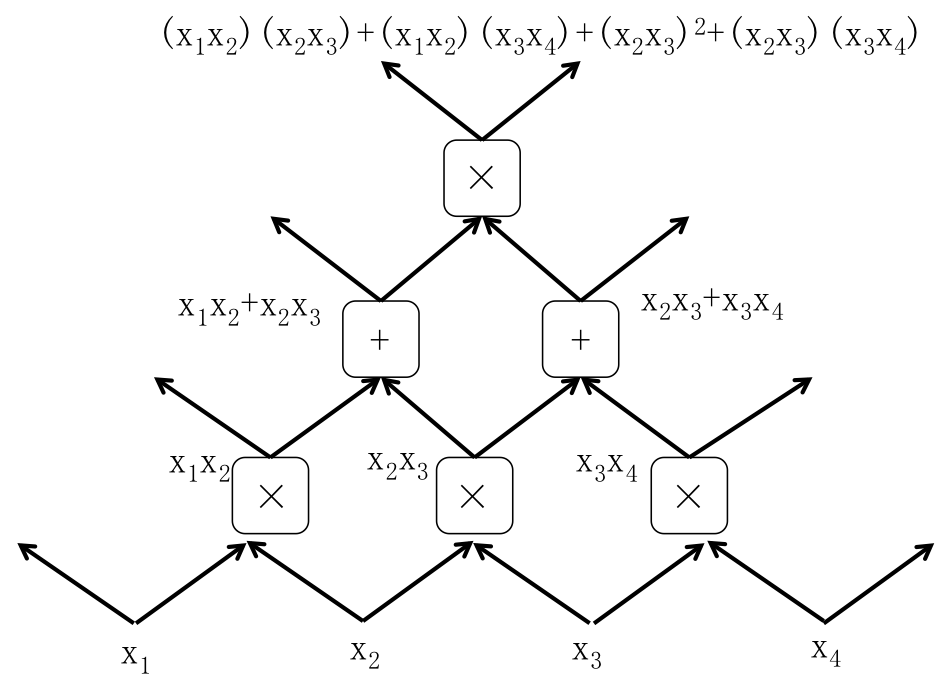
\includegraphics[width=0.7\textwidth]{DANOVA.png}
\caption{The deep structure of DANOVA for feature engineering}
\label{fig:DANOVA}
\end{figure}

As a deep structure, the method called DANOVA \cite{yoshuabengioolivierdelalleau2012,olivierdelalleauyoshuabengio2012} is well effective for feature engineering. It is a greedy combination starting from single features to stepwise feature interactions. The efficiency of feature mining will increase round hundreds times and save plenty of memory for computing. The basic idea is shown in Figure~\ref{fig:DANOVA}.


\begin{figure}[htbp]
\centering
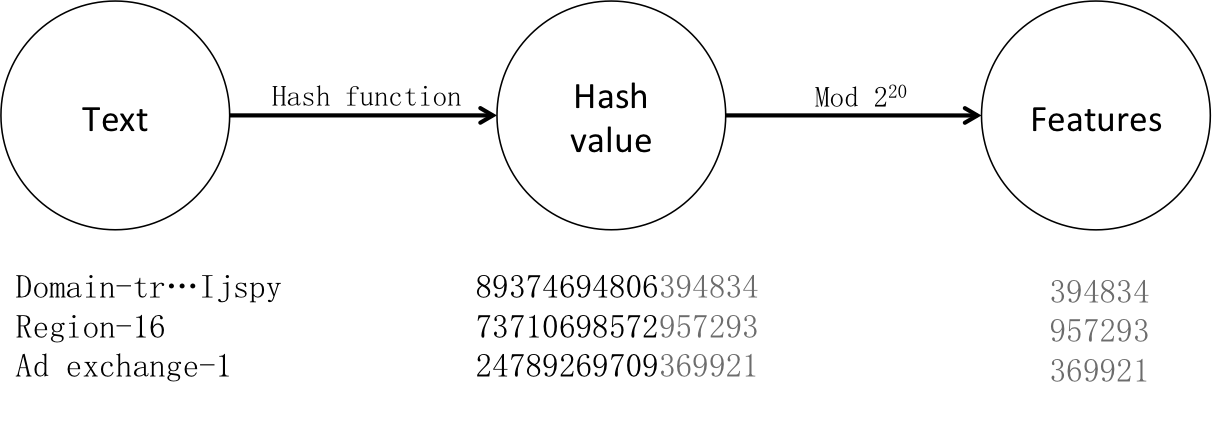
\includegraphics[width=0.8\textwidth]{hashing.png}
\caption{The hashing trick is used to save RAM for computation}
\label{fig:hashing}
\end{figure}

Categorical features appear less than 10 times are transformed into a special value. GBDT features and interaction features based on deep structure are directly included. These groups of features are hashed into $2^{20}$ dimension by hashing trick in Figure~\ref{fig:hashing}. 

Besides, there are some additional ways to generate features: Counting Features, Bag Features, Click History, etc.

\section{Online Learning Algorithms}

iPinYou dataset used in this project is about 16 GB. In terms of a single advertiser, the size of date is still around 2 GB. To the best of our knowledge, it is very difficult to learn model using the whole dataset or mini-batch as the memory in one machine is not enough. Online learning is designed for a sequential data stream. The predictive model is updated after receiving a new data point. It could be used in the case of a process occurring in time. 

The uncertain CTR as an important KPI faces a random distribution of competing bids in each auction. A few online methods can help to estimate its true value. FTRL-proximal online learning algorithm designed by Google is an excellent deterministic and parametric approach to solve large-scale sparsity and convergence issues, but it lacks the prediction of variance of the estimator \cite{h.brendanmcmahangaryholt2013}. Bayesian Online Probit Regression (BOPR) is from Microsoft Bing. It is an online probabilistic way to obtain estimated CTR. The distribution of estimator can be approximated by sampling and updating \cite{thoregraepeljoaquinquinonerocandelathomasborchertralfherbrich2010}. The paper written by Facebook team \cite{xinranhejunfengpanetc2014} gives a comparison between these two methods and also implies the feature engineering insight using Gradient Boosting Decision Trees (GBDT) that can improve the predicting performance. Besides, Field-aware Factorization Machine (FFM) which is widely used in collaborative filtering can provide a new form of estimator \cite{michaeljahrerandreastscherjeongyoonleejingjingdeng2012, steffenrendle2010}. It usually has outperformance than other linear estimator based methods.

\subsection{Bayesian Online Probit Regression (BOPR)}
In this section, we introduction a Bayesian CTR estimation algorithm. We build a generalized linear model with a probit link function to predict CTR. Before illustrating existing models, we introduce some basic notations in Table~\ref{tab:BOPR}:


\begin{table}[H]
\caption{Notation and description of BOPR}
\label{tab:BOPR}
\begin{center}
\begin{tabular}{ l l } 
\hline
Notation & Description \\
\hline
$\mathbf{x}$ & The bid request which is determined by its sparse and binary \\
& feature vector after one-hot encoding\\
$\mathbf{w}$ & The weight which is a linear estimator of probit link function\\
$y$ & Binary label of click \\
$\theta$ & Click-through rate \\
$\bm{\mu }$ & A vector of means of the weight \\
$\bm{\sigma }$ & A vector of variances of the weight \\
$\Sigma$ & Total variance of a given input \\
$s, t$ & Latent variables for factorization density function\\
$f$ & Sample weight from Gaussian prior\\
$g$ & The score $s$ for $\mathbf{x}$ as the inner product\\
$h$ & Factor to obtain $t$ from $s$ by adding zero-mean Gaussian noise \\
$q$ & Click value mapped by a threshold and Sigmoid function \\
\hline
\end{tabular}
\end{center}
\end {table}
After feature transformation, an ad feature becomes a binary encoding vector $\mathbf{x}=(\mathbf{x}_{j1},...,\mathbf{x}_{jk})$ where $\mathbf{x}_{j}$ is the $j$-th discrete feature for all $j\in\left \{ 1,...,J \right \}$ and $j1,...,jk$ are the values of the $k$ categories. We denote the total dimension of $\mathbf{x}$ is $d$. In order to arrive at Bayesian online learning for probit regression (BOPR), the likelihood and prior for advertiser $i$ are given by (we drop $i$ here)
\begin{equation}
\label{samplingprior}
p(y|\mathbf{x},\mathbf{w})=\Phi (\frac{y\cdot \mathbf{w}^{T} \mathbf{x}}{\beta })
\end{equation}
where $\Phi(t)$ is the cumulative density function of standard normal distribution and $N(t)$ is the density function of the standard normal distribution. The parameter $\beta$ scales the steepness of the inverse link function.
\begin{equation}
p(\mathbf{w})=\prod_{j=1}^{J} \prod_{k=1}^{K_j}N(w_{jk},\mu_{jk},\sigma_{jk}^2)
\end{equation}
In terms of the given sampling distribution Eq.~(\ref{samplingprior}), we can obtain the posterior probability of $\mathbf{w}$
\begin{equation}
p(\mathbf{w}|\mathbf{x},y) \propto p(y|\mathbf{x},\mathbf{w}) \cdot p(\mathbf{w})
\end{equation}
The distribution can be interpreted in Figure~\ref{fig:BOPR}.

\begin{figure}[htbp]
\centering
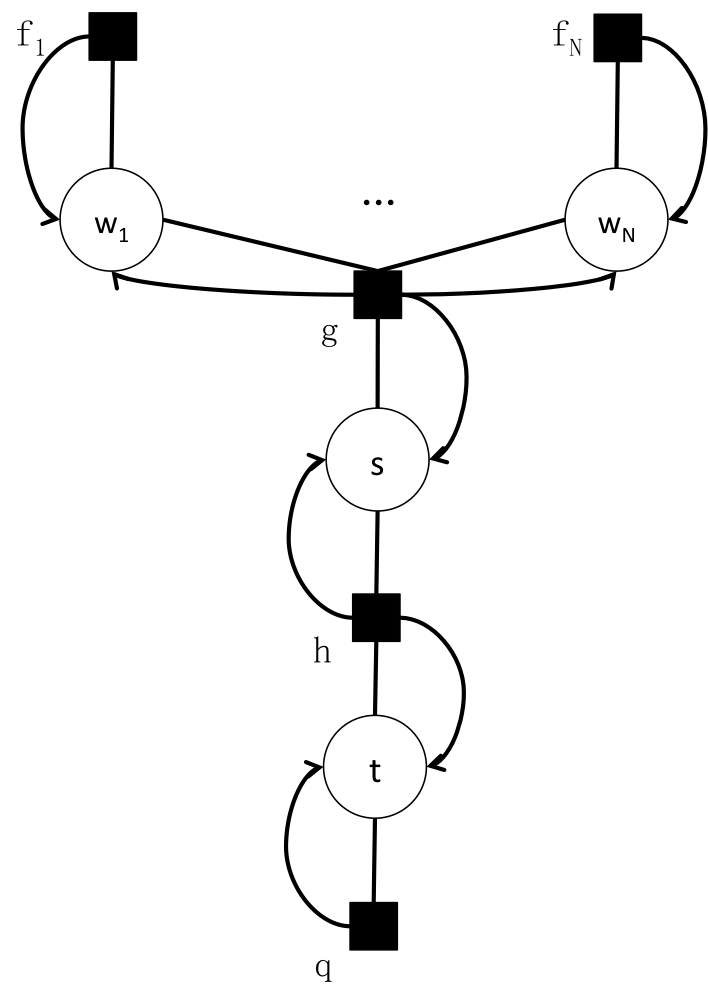
\includegraphics[width=0.5\textwidth]{BOPR.png}
\caption{Factor graph model of BOPR with message flow}
\label{fig:BOPR}
\end{figure}

We introduce two latent variables $t,s$ and three factors $f,g,h$ where $f$ is the sample weights $\mathbf{w}$ from the Gaussian prior, $s=\mathbf{w}^{T}\mathbf{x}$, $g$ gives $p(s|\mathbf{x},\mathbf{w})=\delta (s)$, $h$ adds zero-mean Gaussian noise to obtain $t$ from $s$ such that $p(t|s)=N(t;s,\beta^{2})$ and $q$ is a function such that $p(y|t)=\delta (y=sign (t))$. They satisfy a factorization relation
\begin{equation}
p(y,t,s,\mathbf{w}|t) \propto p(y|t) \cdot p(t|s) \cdot p(s|\mathbf{x},\mathbf{w}) \cdot p(\mathbf{w})
\end{equation}
In this application, the Bayesian online learning algorithm is based on the \emph{Stochastic Gradient Descent} (SGD) or \emph{Online Gradient Descent} (OGD), which attempts to update the posterior distribution of weight vector $\mathbf{w}$. The inference in the algorithm is to approximate $p(\mathbf{w}|y,\mathbf{x})$ and project it back to the closet factorizing Gaussian distribution of $p(\mathbf{w})$. The update equations for parameters $\bm{\mu }$ and $\bm{\sigma }$ are obtained as
\begin{equation}
\hat{\mu }_{{jk}}\leftarrow \mu _{{jk}}+yx_{{jk}}\cdot \frac{\sigma_{{jk}}^{2}}{\Sigma}\cdot \nu (\frac{y \cdot \mathbf{x}^{T}\bm{\mu}}{\Sigma })
\end{equation}
\begin{equation}
\hat{\sigma }^{2}_{{jk}}\leftarrow \sigma ^{2}_{{jk}}\cdot [1-x_{{jk}}\cdot \frac{\sigma_{{jk}}^{2}}{\Sigma ^{2}}\cdot q(\frac{y\cdot \mathbf{x}^{T}\bm{\mu }}{\Sigma })]
\end{equation}
\begin{equation}
\Sigma ^{2} := \beta ^{2}+\sum_{k=1}^{K_{j}}\sigma _{{jk}}^{2}
\end{equation}

\begin{figure}[htbp]
\centering
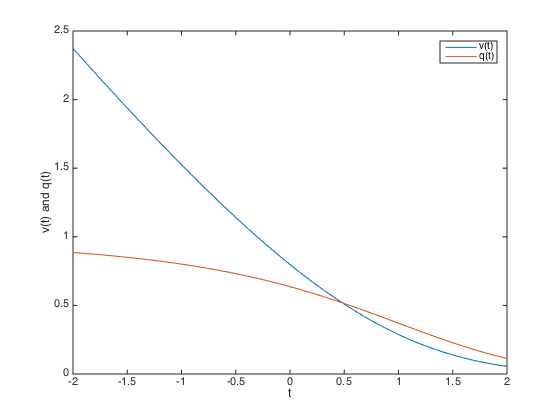
\includegraphics[width=0.8\textwidth]{vandq.png}
\caption{Plot of learning step size function $\nu(t)$ and $q(t)$}
\label{fig:vandq}
\end{figure}

The corrector functions $\nu$ and $q$ are given by $\nu(t):=N(t)/\Phi(t)$ and $q(t):=\nu (t)\cdot [\nu (t)+t]$ in Figure~\ref{fig:vandq}. In the regime $y \cdot \mathbf{x}^{T}\bm{\mu}<0$, the function $\nu(\cdot)$ grows almost linearly which plays a more significant role if errors happen. For the update equations, every observation will result in a decrease in variance of the weight. Therefore, the predictive function is the marginal distribution of the likelihood
\begin{equation}
p(y|\mathbf{x})=\int p(y|\mathbf{x},\mathbf{w})p(\mathbf{w})d\mathbf{w}=\Phi (\frac{y\cdot \mathbf{x}^{T}\bm{\mu}}{\Sigma })
\end{equation}
Comparing with the parameter defined and sampling distribution above, we have the inference result of CTR as
\begin{equation}
\theta=p(y=1|\mathbf{x})=\Phi (\frac{\mathbf{x}^{T}\bm{\mu}}{\Sigma })
\end{equation}
As the number of observation is large enough, the situation that variance converges to zero will occur. The prediction has some similarities as FTRL-Proximal which only considers the weight and ignores the change of variance. If variance is still needed, we can add some techniques like dynamics to generate a correction for variance.

\subsection{Follow the Regularized Leader (FTRL)}

As predicting CTR is a massive-scale learning problem, FTRL-Proximal online learning algorithm with good sparsity and convergence properties can be applied to exploring the dynamic system \cite{h.brendanmcmahan2011}. It will better the memory savings, visualizing performance, confidence estimation and calibration methods. We introduce some basic notations in Table~\ref{tab:FTRL}:
\begin{table}[H]
\caption{Notation and description of FTRL-Proximal}
\label{tab:FTRL}
\begin{center}
\begin{tabular}{ l l } 
\hline
Notation & Description \\
\hline
$\mathbf{x}$ & The bid request which is determined by its sparse and binary \\
& feature vector after one-hot encoding\\
$\mathbf{w}$ & The weight which is a linear estimator of logistic regression \\
$\mathbf{g}$ & The gradient of weight update \\
$y$ & Binary label of click \\
$\theta$ & Click-through rate \\
$t$ & The times of round \\
$\eta$ & A non-increasing learning rate \\
$\lambda$ & Regularization Parameter \\
\hline
\end{tabular}
\end{center}
\end {table}

To present how we can implement FTRL-Proximal precisely,  we also denote the compressed summation notation $\mathbf{g}_{1:t}=\sum_{s=1}^{t}\mathbf{g}_{s}$. We predict $\theta_t=\sigma(\mathbf{w}_t \cdot \mathbf{x}_t)$, where $\sigma(\cdot)$ is a sigmoid function. It can straightforward show the gradient at each round is given by $(\theta-y)\mathbf{x} \in \mathbb{R}^{d}$. However, SGD or OGD is not particularly effective for solving sparse models. To avoid this issue, \emph{Elastic Net} adds $L1$ regularization (known as Lasso) and $L2$ regularization (known as Ridge) to trade-off the degree of sparsity. By \emph{Following the Regularized Leader} (FTRL), the online gradient descent perform a update
\begin{equation}
\mathbf{w}_{t+1}=\mathbf{w}_{t}-\eta _{t} \cdot \mathbf{g}_{t}
\end{equation}

The learning rate is non-increasing. In order to be adaptive based on historical gradient, it is defined by
\begin{equation}
\eta _{t,i}=\frac{\alpha}{\beta + \sqrt{\sum_{s=1}^{t}g_{s,i}^{2}}}
\end{equation}
Hence, the FTRL-Proximal algorithm uses the update formulation given below
\begin{equation}
\label{FTRL}
\mathbf{w}_{t+1}=\underset{\mathbf{w}}\argmax (\mathbf{g}_{1:t} \cdot \mathbf{w} + \frac{1}{2}\sum_{s=1}^{t}\sigma_{s}\left \|\mathbf{w}-\mathbf{w}_s  \right \|_{2}^{2}+\lambda_{1}\left \|\mathbf{w}  \right \|_{1})
\end{equation}
where $\sigma_{1:t}=\frac{1}{\eta _{t}}$. This update seems to require storing all the past coefficients. It will lead to lower time sensitivity and looks much more complicated than common gradient descent. However, the memory can be saved indeed because we only need to store only one number per coefficient. The Eq.~(\ref{FTRL}) is rewritten as the argmin over $\mathbf{w} \in \mathbb{R}^{d}$ of
\begin{equation}
(\mathbf{g}_{1:t}-\sum_{s=1}^{t}\eta _{t}\mathbf{w}_{s})\cdot \mathbf{w}+\frac{1}{\eta _{t}}\left \|\mathbf{w} \right \|_{2}^{2}+ \lambda _{1} \left \|\mathbf{w}  \right \|_{1}+(const)
\end{equation}

Thus, if we store $\mathbf{z}_{t-1}=\mathbf{g}_{1:t-1}-\sum_{s=1}^{t-1}\sigma_{s}\mathbf{w}_{s}$ at the beginning of round $t$, we can add an intermediate substitution expressed by $\mathbf{z}_{t}$. The update lets
\begin{equation}
\mathbf{z}_{t}=\mathbf{z}_{t-1}+\mathbf{g}_{t}+(\frac{1}{\eta_t}-\frac{1}{\eta_{t-1}})\mathbf{w}_{t}
\end{equation}
and solve for $\mathbf{w}_{t+1}$ in closed form on a per-coordinate bases by
\begin{equation}
w_{t+1,i}=\left\{\begin{matrix}
0 &\mathrm{if } |z_{t,i}| \leq \lambda_{1} \\ 
 -\eta_t(z_{t,i}-sign(z_{t,i})\lambda_1) & \mathrm{otherwise}
\end{matrix}\right.
\end{equation}
It implies that only $\mathbf{z}_t$ needs to be stored in memory and we do not need to store the historical gradient since we can use $\mathbf{z}_t$ to show the previous situations. When $\lambda_1=0$, it transforms to be 
\begin{equation}
\mathbf{w}_{t+1} = -\eta_t \mathbf{z}_{t}=-\eta_t \sum_{s=1}^{t}\mathbf{g}_s
\end{equation}
In this case, the memory cost is exactly same as the normal gradient descent coefficient. Nevertheless, there is no free lunch. Even though FTRL-Proximal can deal with large-scale sparsity properly, it still has shortcomings comparing with BOPR. It is too complicated to generate a variance for the estimator because it is a deterministic approach.

\subsection{Field-aware Factorization Machine (FFM)}
The idea of FFM is firstly used in \emph{Collaborative Filtering} (CF) since the data table consisting of both fields and features. A technique called \emph{Alternative Least Squares} (ALS) is very applicable for the decomposition of association matrix and learning of latent factors. Estimation of CTR also can be treated as a FFM problem. We introduce some basic notations in Table.~\ref{tab:FFM}:
\begin{table}[H]
\caption{Notation and description of FFM}
\label{tab:FFM}
\begin{center}
\begin{tabular}{ l l } 
\hline
Notation & Description \\
\hline
$\mathbf{x}$ & The bid request which is a numerical feature vector\\
$\mathbf{w}$ & The weight which is a field  estimator \\
$\phi$ & The mapping function \\
$y$ & Binary label of click \\
$\theta$ & Click-through rate \\
\hline
\end{tabular}
\end{center}
\end {table}

The commonly applied mapping approaches for regression are like first order Linear Model and Degree-2 Polynomial Model . The feature mapping functions like those in \emph{Support Vector Machine} (SVM) are given by
\begin{itemize}
  \item Linear Model:
	\begin{equation}
	\phi (\mathbf{w},\mathbf{x})=\sum_{j \in C}w_{j}x_{j}
	\end{equation}
  \item Degree-2 Polynomial Model (Ploy2):
	\begin{equation}
	\phi (\mathbf{w},\mathbf{x})=\sum_{j_1,j_2 \in C}{w}_{j_1, j_2}x_{j_1}x_{j_2}
	\end{equation}
\end{itemize}
In the above situations, the weight as coefficient is a scalar value for the single feature vector or the interaction of different feature vectors.  However, based on the well known regression models, for \emph{Factorization Machine} (FM) \cite{michaeljahrerandreastscherjeongyoonleejingjingdeng2012}, the form is more extensive. The current coefficient is the inner product of weight vectors. The weight vector $\mathbf{w} \in \mathbb{R}^{d} $ is a latent factor used to describe the fields and features. The mathematical formulations for FM and FFM \cite{steffenrendlelarsschmidtthieme2010} are
\begin{itemize}
	\item Factorization Machines (FM):
		\begin{equation}
		\phi (\mathbf{w},\mathbf{x})=\sum_{j_1,j_2 \in C}<\mathbf{w}_{j_1},\mathbf{w}_{j_2}>x_{j_1}x_{j_2}
		\end{equation}
	\item Field-aware Factorization Machines (FFM):
		\begin{equation}
		\phi (\mathbf{w},\mathbf{x})=\sum_{j_1,j_2 \in C}<\mathbf{w}_{j_1,f_2},\mathbf{w}_{j_2,f_1}>x_{j_1}x_{j_2}
		\end{equation}		
\end{itemize}

Let us show a concrete FFM example of overall CTR estimation in practice, which only includes three advertiser fields and five ad features. We want to map categorical values into corresponding field indexes and feature indexes. The mapping relationship is in Table~\ref{tab:FFMCTR}.

\begin{table}[H]
\caption{A concrete FFM example of overall CTR estimation in practice}
\label{tab:FFMCTR}
\begin{tabular}{ p{3cm}p{3cm}|p{3cm}p{3cm}  }
 \hline
 \multicolumn{4}{c}{Fields and Features Mapping} \\
 \hline
Field Name & Field Index & Feature Name & Feature Index \\
 \hline
Ader ID-1458  & field \color{red}{1}    & UserAgent-window-chrome &  feature \color{blue}{5}\\
Ader ID-2259 & field \color{red}{2}  & City-11  & feature \color{blue}{8}\\
AderID-2261 & field \color{red}{3} & Ad slot format-1 & feature \color{blue}{17}\\
 & & Region-16 & feature \color{blue}{5} \\
  & & UserTags-10006 & feature \color{blue}{6} \\
 \hline
\end{tabular}
\end{table}

After transformation to the FFM format, the encoding of data raises as 
\begin{center}
\color{red}{1}:\color{blue}{5}:\color{black}{1}	\color{red}{2}:\color{blue}{8}:\color{black}{0}	\color{red}{3}:\color{blue}{17}:\color{black}{1}	\color{red}{2}:\color{blue}{5}:\color{black}{1}	\color{red}{1}:\color{blue}{6}:\color{black}{1}
\end{center}
For FFM, $\phi (\mathbf{w},\mathbf{x})$ is
\begin{equation}
\begin{split}
& <\mathbf{w}_{\color{red}{1},\color{blue}{5}}, \mathbf{w}_{\color{red}{2},\color{blue}{8}}> \cdot {1} \cdot 0 + <\mathbf{w}_{\color{red}{1},\color{blue}{5}}, \mathbf{w}_{\color{red}{3},\color{blue}{17}}> \cdot 1 \cdot 1 + <\mathbf{w}_{\color{red}{1},\color{blue}{5}}, \mathbf{w}_{\color{red}{2},\color{blue}{5}}> \cdot 1 \cdot 1 + <\mathbf{w}_{\color{red}{1},\color{blue}{5}}, \mathbf{w}_{\color{red}{1},\color{blue}{6}}> \cdot 1 \cdot 1 \\
& <\mathbf{w}_{\color{red}{2},\color{blue}{8}}, \mathbf{w}_{\color{red}{3},\color{blue}{17}}> \cdot 0 \cdot 1 + <\mathbf{w}_{\color{red}{2},\color{blue}{8}}, \mathbf{w}_{\color{red}{2},\color{blue}{5}}> \cdot 0 \cdot 1 + <\mathbf{w}_{\color{red}{2},\color{blue}{8}}, \mathbf{w}_{\color{red}{1},\color{blue}{6}}> \cdot 0 \cdot 1 \\
& <\mathbf{w}_{\color{red}{3},\color{blue}{17}}, \mathbf{w}_{\color{red}{2},\color{blue}{5}}> \cdot 1 \cdot 1 + <\mathbf{w}_{\color{red}{3},\color{blue}{17}}, \mathbf{w}_{\color{red}{1},\color{blue}{6}}> \cdot 1 \cdot 1 \\
& <\mathbf{w}_{\color{red}{2},\color{blue}{5}}, \mathbf{w}_{\color{red}{1},\color{blue}{6}}> \cdot 1 \cdot 1
\end{split}
\end{equation}
Unlike nonlinear SVMs, a transformation in the dual form is not necessary and the model parameters of FFM can be estimated directly without the need of any support vector. Also, FFM has the advantages in sparse settings \cite{steffenrendle2010}. Besides feature interactions, first order features are also used in FFM model. Thus, the optimization problem is
\begin{equation}
\underset{\mathbf{w}}{\min}\frac{1}{L} \sum_{i=1}^{L}(\log (1+\exp (-y_i \phi (\mathbf{w}, \mathbf{x}_i)))+\frac{\lambda}{2}\left \| \mathbf{w} \right \|^{2})
\end{equation}
where 
\begin{equation}
\phi (\mathbf{w},\mathbf{x})=\sum_{j_1,j_2 \in C}<\mathbf{w}_{j_1,f_2},\mathbf{w}_{j_2,f_1}>x_{j_1}x_{j_2}+\sum_{j \in C}w_{j}x_{j}
\end{equation}
The results of FM and FFM are identical or very similar to many of the specialized state-of-the-art models.











\chapter{Auction Theory}
\label{chapterlabel3}

In this chapter, we discuss the basic auction theory which is used in online advertising. The most commonly applied auction is sealed first-price bid and sealed second-price bid. According to the closed form solutions of these two kinds of auction as games, there are two conclusions to the bidding strategy based on the true value. 

\section{Bayesian Nash Equilibrium}
Bayesian Nash Equilibrium is firstly defined by Harsanyi \cite{johncharsanyi1967}. For each auction, the participant only knows their own type, but they do not know other players' types. The type here means the input value of their strategies. In a scenario of real-time bidding, it can be the true value or signal of each ad for advertisers. True value is the belief that what is the real worth of this ad. All advertisers will bid a price based on their own true value. The way mapping from the set of possible types to the bidding price is called bidding strategy. In an auction, the basic environment consists of:
\begin{itemize}
\item One object to be sold
\item A set of independent and identical bidders $\bs{I} = \{ 1,2,...,N\}$
\item A set of possible independent types or signals $\theta_1, \theta_2,...,\theta_N$ and $\theta_i \in [\underline{\theta}, \bar{\theta}]$
\item A set of bidding strategies $B_1, B_2,...,B_N$ for each bidder
\item A utility (or reward) function $u_i$ for bidder $i$ 
\item A cumulative distribution $F(\cdot)$ over the set of types for each bidder
\end{itemize}
In  short, a \emph{Bayesian Game} in ad campaign context consists of five elements which can be expressed as a tuple:
\begin{equation}
BG=[\bm{I}, \{ B_i \}_{i \in \bm{I}}, \{ u_{i}(\cdot) \}_{i \in \bm{I}},  \theta_1 \times \cdot \cdot \cdot \times \theta_N, F(\cdot)]
\end{equation}

Further, a \emph{Bayesian Nash equilibrium} is a list of bidding functions $(b_{1}^{*}(\cdot),...,b_{N}^{*}(\cdot))$. For $\forall i \in \bm{I}, \forall \theta_i$ and $\forall b_i \in B_i$, it has
\begin{equation}
\int_{\theta_-i}u(b_{i}^{*}, b_{-i}^{*}, \theta_{i}, \theta_{-i})d\hat{F}_{i}(\theta_{-i}|\theta_{i}) \geq \int_{\theta_-i}u(b_{i}, b_{-i}^{*}, \theta_{i}, \theta_{-i})d\hat{F}_{i}(\theta_{-i}|\theta_{i})
\end{equation}
where notations denote $\theta_{-i} \equiv (\theta_{j})_{j \neq i}$ and $\hat{F}_{i}(\theta_{-i})=F_{1}(\theta_1)\cdot \cdot \cdot F_{i-1}(\theta_{i-1})F_{i+1}(\theta_{i+1})\cdot \cdot \cdot F_{N}(\theta_{N})$.

Accord to the Nash equilibrium inequality applying Bayesian decision function, it implies the situation that each bidder has a best response strategy and choose the best Bayesian decision functions based on the best bidding strategies of other bidders. They also use the Bayesian decision functions to determine their response. This Nash equilibrium is not necessary to be unique in an auction environment. Besides, if all players use the same decision function, we call this a \emph{symmetric Bayesian Nash equilibrium}. In the following sections, we use this setting for all games of incomplete information and we assume that all bidders are identical and independent.
\section{Auction as Games}
In this section, a brief of introduction to auction will be provided. Auction can be basically classified into four forms with regard to several distinct criteria.They are English, Dutch, First-Price, and Vickrey auctions respectively. 

The English or publicly ascending-price auction is the best-known format. It begins as a low price and bidders incrementally increase the price. Once no other bidder is willing to give a higher price, the auction stops and the bidder with the highest standing price wins the bid and pays the highest price. 

Dutch is kind of open descending-price auction which conducts in the opposite way. Bidding starts at a high price that continuously declines until one of the bidders stops the process. That participant wins the object and pays the stopped price.

In terms of Vickrey auction, the only difference is that bidder with the highest price wins the bid and pays the second highest price in the market. For both first-price and second-price sealed-bid auction, each player does not have the knowledge of the bids proposed by others. They only can obtain information from the market after winning or losing the bid. 

The objective of each bidder is to maximize the utility of the auction or campaign. Once players determine their intuitive true value and bidding price, the utility is the expected difference between the two which can be positive or negative. In a one-shot auction, we usually assume that player's bidding price will not exceed his true value since there is no \emph{exploitation-exploration} trade-off.

Decision making in repeated games contains two fundamental choices. Exploration is to sacrifice current benefit to gather more information which may better the performance in the future. It is long-term, risky and uncertain. The best long-term and overall strategy may involve short-term loss. In the contrary, exploitation process is short-term, immediate and gives certain benefits. 

In this project, we mainly focus on Real-time Bidding (RTB). RTB is a form of auction game. Unlike traditional sponsored search or contextual advertising, RTB allows an advertiser to submit a bid for each individual impression or keyword campaign in a short time frame. Sponsored search is more like a multi-bandit problem, the number of objects is more than one and a mechanism for ranking the bids is involved. The approach to deal with exploitation and exploration in repeated games will be introduced in detail in Chapter 4.

\section{Sealed First-price Auction}
In a sealed first-price auction, bidders will submit their bids $b_1,...,b_N$ and they do not know others' price. Under this setting, if bidders submit their true value, they will earn a zero profit or utility no matter whether they win or lose. Intuitively, they should bid a price somewhat lower than the corresponding true value and then it can potentially provide a positive utility when winning the bid.

In a more theoretical perspective, we consider an approach to solve the symmetric equilibrium bidding strategies. Assume that the bidding strategy is a strictly increase function. It indicates that higher true value will lead to higher bid. Also, suppose that bidder $j \neq i$ follows identical bidding strategies $b_j=b(\theta_j)$ with the above properties. Therefore, the utility of bidder $i$ for one-shot auction can be expressed as 
\begin{equation}
u(b_i,\theta_i)=(\theta_i-b_i) \cdot \Pr [b_j=b(\theta_j)\leq b_i, \forall j \neq i]
\end{equation}
In order to maximize the utility by choosing an optimal bidding strategy, we can obtain the objective. Thus, bidder $i$ chooses $b$ to solve
\begin{equation}
\label{objective}
\underset{b_i} \max (\theta_i-b_i)F^{N-1}(b^{-1}(b_i))
\end{equation}
Differentiate Eq.~(\ref{objective}) with respect to $b_i$ and let it be zero. The first order condition becomes
\begin{equation}
(\theta_i-b_i)(N-1)F^{N-2}(b^{-1}(b_i))f(b^{-1}(b_i))\frac{1}{b'(b^{-1}(b_i))}-F^{N-1}(b^{-1}(b_i))=0
\end{equation}
As a symmetric equilibrium, $b_i=b(\theta_i)$, so the first order condition transforms to a differential equation 
\begin{equation}
b'(\theta_i)=(\theta_i-b(\theta_i))(N-1)\frac{f(\theta_i)}{F(\theta_i)}
\end{equation}
This can be solved, using the boundary condition that $b(\underline{\theta})=\underline{\theta}$, to obtain
\begin{equation}
\label{biddingfirst}
b^{*}(\theta_i)=\theta_i-\frac{\int_{\underline{\theta}}^{\theta_i}F^{N-1}(\widetilde{\theta})d\widetilde{\theta}}{F^{N-1}(\theta_i)}
\end{equation}
As we assume the $b(\theta_i)$ is increasing and differentiable. The symmetric equilibrium shows that arbitrary bidder in this auction can use Eq.~(\ref{biddingfirst}) to find his optimal bidding strategy. A closely related, and often convenient, approach to identify necessary conditions for a symmetric equilibrium is to exploit the envelope theorem.
\begin{equation}
\label{envelope}
u(\theta_i)=(\theta_i-b(\theta_i))F^{N-1}(\theta_i)
\end{equation}
Likewise, we can find a best-response in the equilibrium for bidder $i$
\begin{equation}
u(\theta_i)=\underset{b_i} \max (\theta_i-b_i)F^{N-1}(b^{-1}(b_i))
\end{equation}
After applying the envelope theorem \cite{milgrompaililyasegal2002}, we obtain
\begin{equation}
\frac{d}{d \theta}u(\theta)|_{\theta_i}=F^{N-1}(b^{-1}(b(\theta_i)))=F^{N-1}(\theta_i)
\end{equation}
and also,
\begin{equation}
\label{envelope2}
u(\theta_i)=u(\underline{\theta})+\int_{\underline{\theta}}^{\theta_i}F^{N-1}(\tilde{\theta})d\tilde{\theta}
\end{equation}
We have $u(\underline{\theta})=0$ because we cannot bid a negative value. Take Eq.~(\ref{envelope}) and Eq.~(\ref{envelope2}) into consideration, we can solve the Bayesian equilibrium situation and obtain the optimal bidding strategy as
\begin{equation}
\label{biddingfirst2}
b^{*}(\theta_i)=\theta_i-\frac{\int_{\underline{\theta}}^{\theta_i}F^{N-1}(\widetilde{\theta})d\widetilde{\theta}}{F^{N-1}(\theta)}
\end{equation}
Hence, Eq.~(\ref{biddingfirst2}) is the same as Eq.~(\ref{biddingfirst}) given the condition for a Bayesian equilibrium. The envelope formula actually satisfies bidding assumptions. The value of shading is therefore $\int_{\underline{\theta}}^{\theta_i}F^{N-1}(\widetilde{\theta})d\widetilde{\theta}$. Obviously, it declines as the number of bidders increases. Intrinsically, if there are a large number of opponents ($N \rightarrow \infty $) in the auction, they have to bid as close as possible to their true value ($b_i \rightarrow \theta_i$). Otherwise, they do not have any chance to win \cite{robertwilson1977}.

\section{Sealed Second-price Auction}
In a sealed second-price auction, the procedure is similar as corresponding first-price auction. All bidders submit their bid simultaneously without observing others' bids. In such scenario, the winner is who submitted the highest price and he only needs to pay the second highest price in the market. The paying price is also called market price. Even though bidder submits his true value every time, he still can obtain a positive utility. If he wins, the second highest price cannot be more than his bid. Meanwhile, if he loses, the utility stays as zero. Thus, bidding true value should result in a positive utility. We will formally prove this strategy is the optimal for second-price sealed-bid auction.

Denote $\theta_t$ is the highest price of other bidder $j$ where $j \neq i$. From bidder $i$'s view, as he does not know other bidders' price, he can only know the expected utility which is written as
\begin{equation}
\label{ExU}
u(b_i, \theta_i) = E [ (\theta_i - \theta_t) \bm{I}_{b_{i} > \theta_t} ]
\end{equation}
where $\bm{I}_{b_{i} > \theta_t}$  denotes an indicator to identify the probability of achieving the highest price in this round. It implies when the bidder can win the auction. Therefore, we can rewrite expected utility Eq.~(\ref{ExU}) in detail to obtain
\begin{equation}
\label{secondprice}
u(b_i, \theta_i)=\int_{\underline{\theta}}^{b_i}(N-1)(\theta_i-\theta_t)f(\theta_t)F(\theta_t)^{N-2}d\theta_t
\end{equation}
Because there are $N-1$ other bidders. The cumulative distribution function of the highest among $N-1$ players is given by $F^{N-1}(\cdot)$.
In order to maximize Eq.~(\ref{secondprice}), if $b_i$ is smaller than $\theta_i$, there is a amount  of increase in the integration
\begin{equation}
\int_{b_i}^{\theta_i}(N-1)(\theta_i - \theta_t)f(\theta_t)F(\theta_t)^{N-2}d\theta_t
\end{equation}
Now, if $b_i < \theta_t < \theta_i$, the above integration is positive as $\theta_i-\theta_t > 0$. On the contrary, if $b_i > \theta_t > \theta_i$, this region gives a negative value. Hence, the maximum of expected utility can be achieved when $b_i=\theta_i$. Based on this integration, a revenue equivalence property can be proved to show first-price and second-price have the same expected revenue for the same object and participants but different mechanisms \cite{menezes2005introduction}.

In summary, bidding true value is the optimal strategy for second-price auction. 





\include{Conclusions}
\addcontentsline{toc}{chapter}{Appendices}

% The \appendix command resets the chapter counter, and changes the chapter numbering scheme to capital letters.
%\chapter{Appendices}
\appendix
\chapter{Dataset and Repository}
The iPinYou dataset can be downloaded from  \\
\url{http://data.computational-advertising.org} \\
The repository of the project can be downloaded from \\
\url{https://github.com/kevinhsu/MSc-project.git} \\
 
 % description of document, e.g. type faces, TeX used, TeXmaker, packages and things used for figures. Like a computational details section.
% e.g. http://tex.stackexchange.com/questions/63468/what-is-best-way-to-mention-that-a-document-has-been-typeset-with-tex#63503

% Side note:
%http://tex.stackexchange.com/questions/1319/showcase-of-beautiful-typography-done-in-tex-friends 
% You could separate these out into different files if you have
%  particularly large appendices.

% This line manually adds the Bibliography to the table of contents.
% The fact that \include is the last thing before this ensures that it
% is on a clear page, and adding it like this means that it doesn't
% get a chapter or appendix number.
\addcontentsline{toc}{chapter}{Bibliography}

% Actually generates your bibliography.
\bibliography{example.bib}

% All done. \o/
\end{document}
